The second question of the survey asks Android developers the programming language or programming languages they use to develop Android applications. As mentioned in section 2, different programming languages can be used while developing Android applications. Nevertheless, this study focuses solely on "Native" Android development, as mentioned many times before. Therefore, only Java and Kotlin programming languages are among the options offered to answer the second question.
\begin{figure}[ht!]
    \centering
    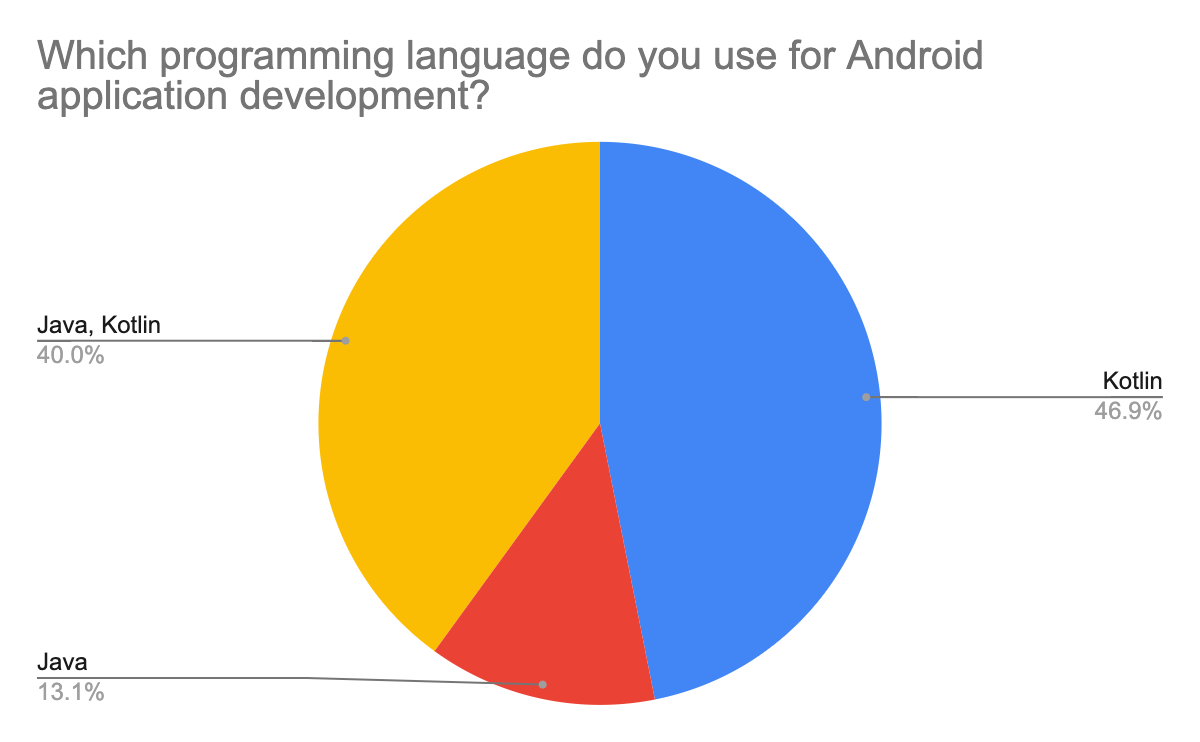
\includegraphics[scale=0.3]{figures/programming_language.png}
    \caption{Programming languages results}
    \label{fig:programming_languages}
\end{figure}

In Fig. \ref{fig:programming_languages} above, Android developers' trends regarding the programming language they use while developing "Native" Android applications can be seen. Around 47\% of the Android developers surveyed seem to use the Kotlin programming language. 40\% of the participants use Java and Kotlin together, while only 13.1\% use the Java programming language. Considering that Kotlin is a programming language suggested by Google and Android and is more "programmer-friendly" than Java, it is not difficult to understand that the above table is not surprising. As of 2020, Google declared that more than 60\% of Android applications were developed with Kotlin. It can be said that the survey results largely overlap with this statement\footnote{\url{https://developer.android.com/kotlin}}. On the other hand, he fact that some users still use Java can be explained by the existence of Android applications developed with Java before Kotlin was declared as an official programming language for Android.

As stated in section \ref{section:4.3}, Mooncascade's Android team develops Android applications using Kotlin programming language, unless otherwise requested by its customers. When the survey results presented in detail above and the company's choice are compared, it is seen that this choice coincides with the Android community’s current trends.